\section{How do GANs work?}

We have now seen several other generative models and explained that GANs do not
work in the same way that they do. But how do GANs themselves work?

\subsection{The GAN framework}

The basic idea of GANs is to set up a game between two players.
One of them is called the \newterm{generator}.
The generator creates samples that are intended to come from the
same distribution as the training data.
The other player is the \newterm{discriminator}.
The discriminator examines samples to determine whether they are real
or fake.
The discriminator learns using traditional supervised learning techniques,
dividing inputs into two classes (real or fake).
The generator is trained to fool the discriminator.
We can think of the generator as being like a counterfeiter, trying to
make fake money, and the discriminator as being like police, trying to
allow legitimate money and catch counterfeit money.
To succeed in this game, the counterfeiter must learn to make money that
is indistinguishable from genuine money, and the generator network must
learn to create samples that are drawn from the same distribution as the
training data.
The process is illustrated in \figref{fig:framework}.

\begin{figure}
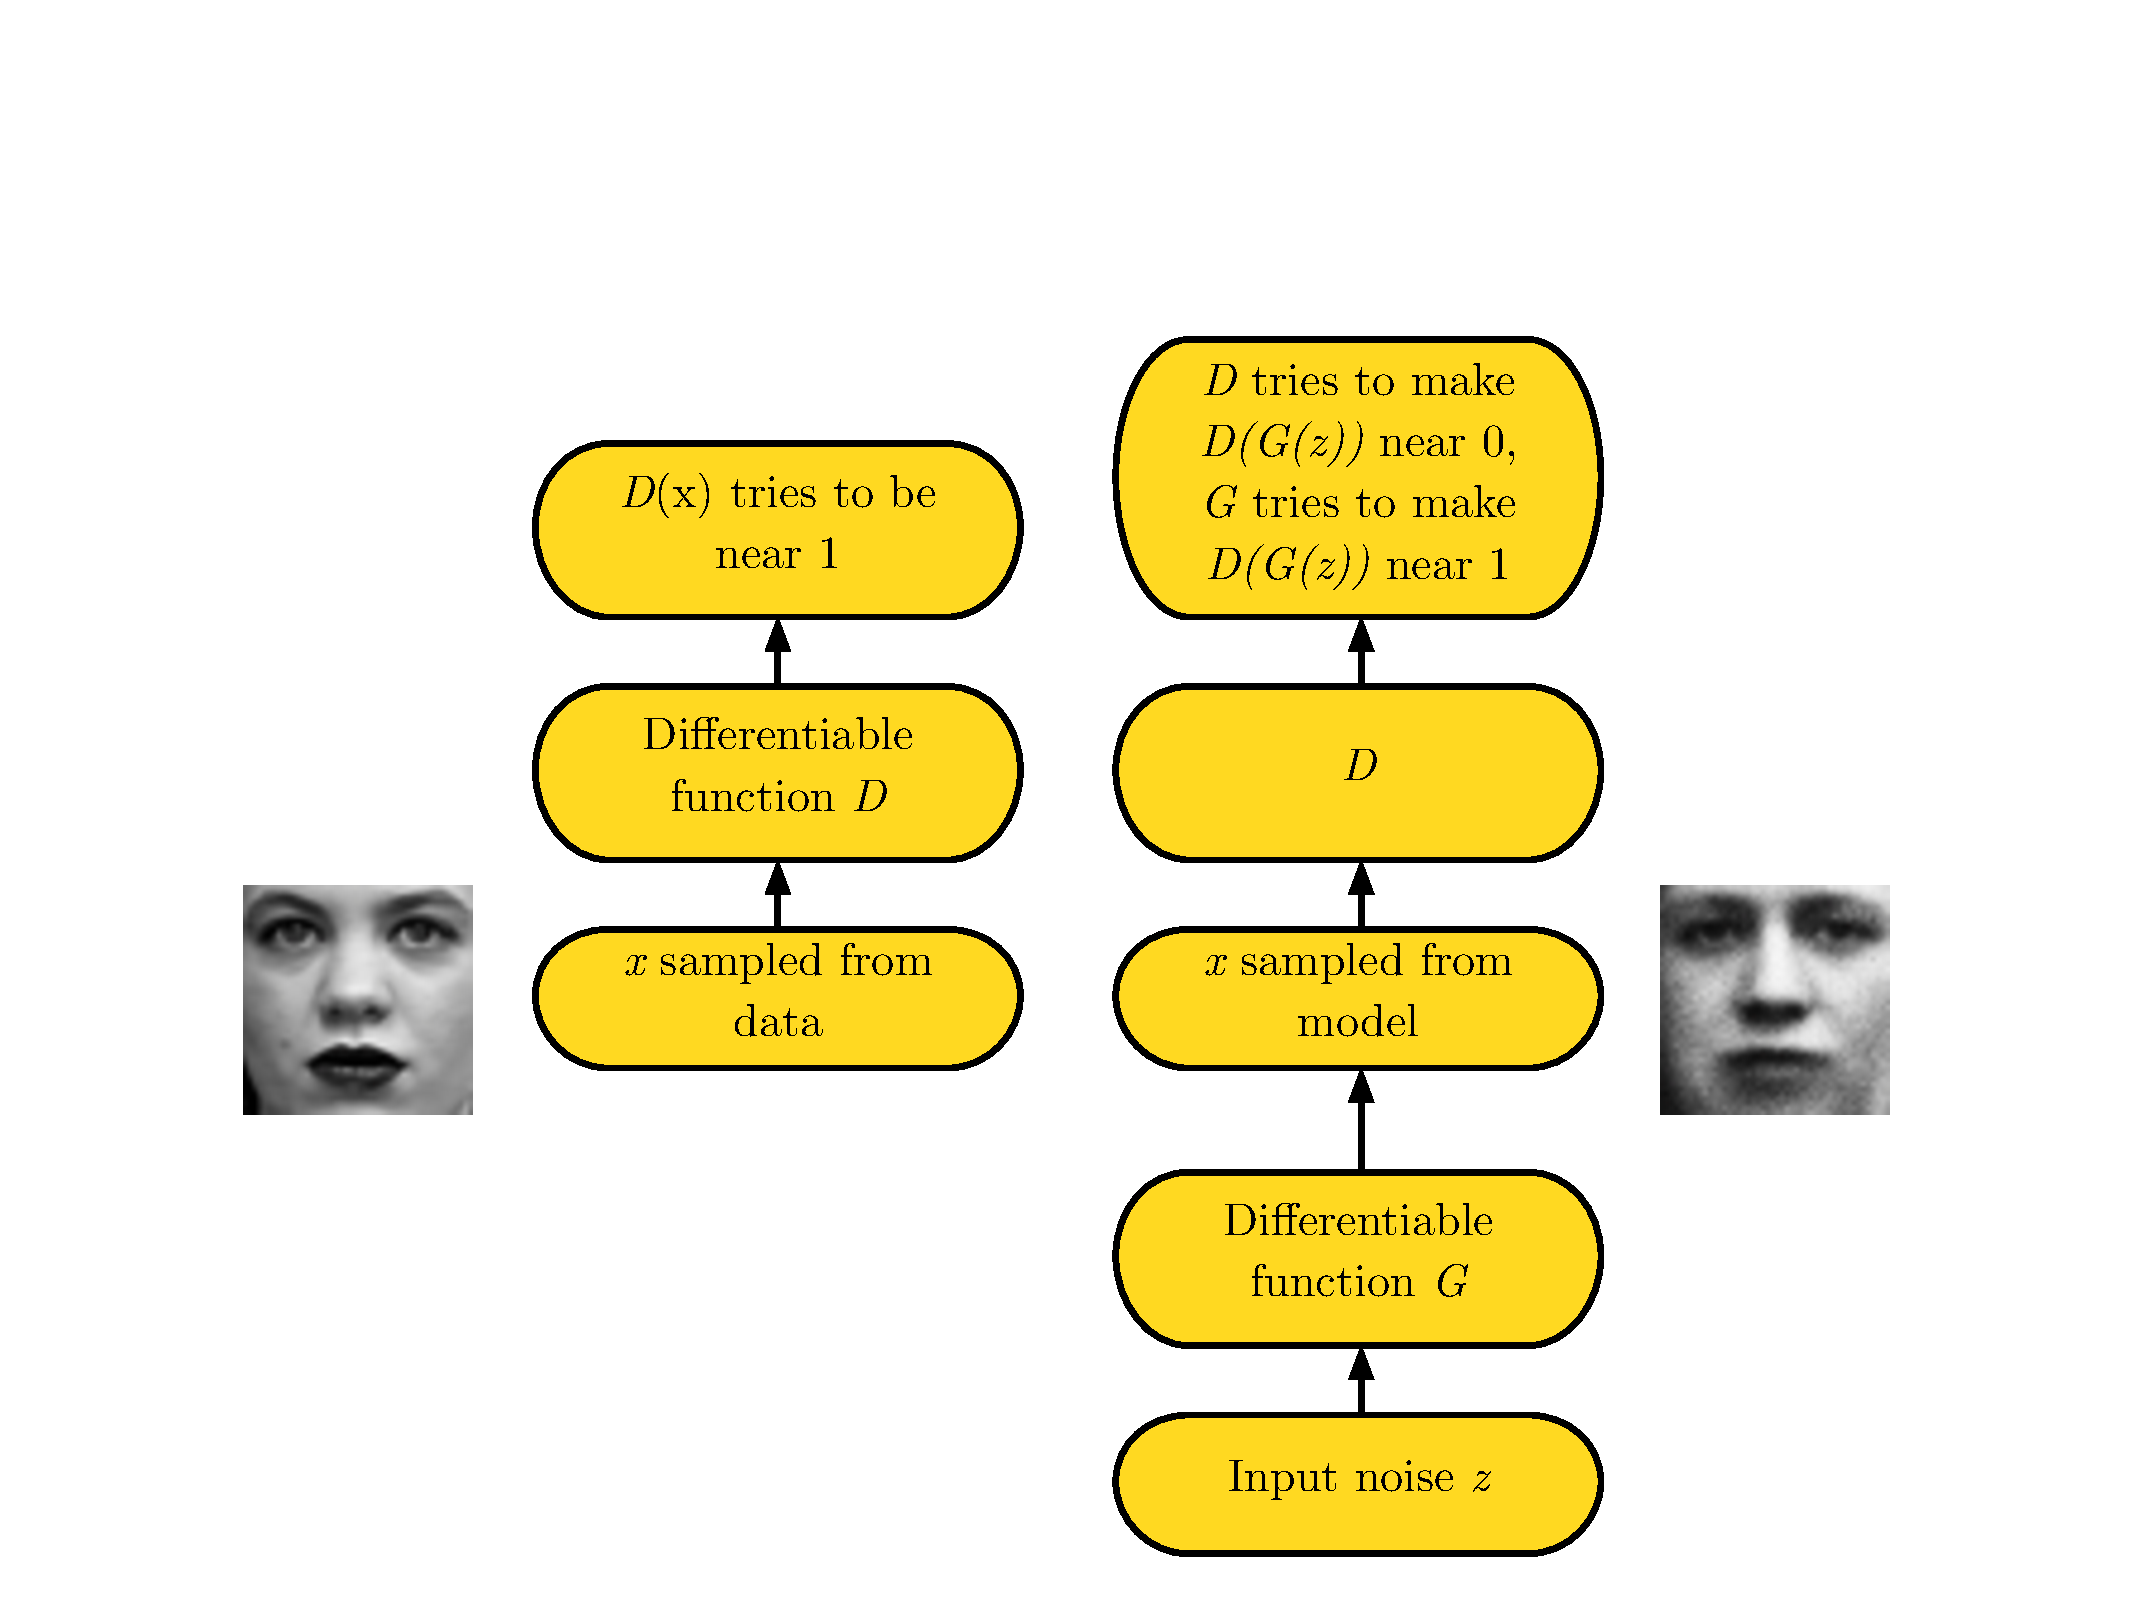
\includegraphics[width=\textwidth]{framework}
\caption{The GAN framework pits two adversaries against each other in a game.
Each player is represented by a differentiable function controlled by a set
of parameters.
Typically these functions are implemented as deep neural networks.
The game plays out in two scenarios.
In one scenario, training examples $\vx$ are randomly sampled from the training
set and used as input for the first player, the discriminator, represented
by the function $D$. The goal of the discriminator is to output the probability
that its input is real rather than fake, under the assumption that half of the
inputs it is ever shown are real and half are fake.
In this first scenario, the goal of the discriminator is for $D(\vx)$ to be
near 1.
In the second scenario, inputs $\vz$ to the generator are randomly sampled from
the model's prior over the latent variables.
The discriminator then receives input $G(\vz)$, a fake sample created by the
generator.
In this scenario, both players participate. The discriminator strives to make
$D(G(z))$ approach 0 while the generative strives to make the same quantity
approach 1.
If both models have sufficient capacity, then the Nash equilibrium of this game
corresponds to the $G(\vz)$ being drawn from the same distribution as the training
data, and $D(\vx) = \frac{1}{2}$ for all $\vx$.
}
\label{fig:framework}
\end{figure}

Formally, GANs are a structured probabilistic model (see chapter 16 of
\citet{Goodfellow-et-al-2016} for an introduction to structured probabilistic
models) containing latent variables $\vz$ and observed variables $\vx$.
The graph structure is shown in \figref{fig:graph}.

The two players in the game are represented by two functions, each of which
is differentiable both with respect to its inputs and with respect to its
parameters.
The discriminator is a function $D$ that takes $\vx$ as input and uses
$\vtheta^{(D)}$ as parameters.
The generator is defined by a function $G$ that takes $\vz$ as input and
uses $\vtheta^{(G)}$ as parameters.

Both players have cost functions that are defined in terms of both players'
parameters.
The discriminator wishes to minimize $J^{(D)}\left( \vtheta^{(D)}, \vtheta^{(G)} \right)$
and must do so while controlling only $\vtheta^{(D)}$.
The generator wishes to minimize $J^{(G)}\left( \vtheta^{(D)}, \vtheta^{(G)} \right)$
and must do so while controlling only $\vtheta^{(G)}$.
Because each player's cost depends on the other player's parameters, but each player
cannot control the other player's parameters, this scenario is most
straightforward to describe as a game rather than as an optimization problem.
The solution to an optimization problem is a (local) minimum, a point in parameter space
where all neighboring points have greater or equal cost.
The solution to a game is a Nash equilibrium.
Here, we use the terminology of local differential Nash equilibria \citep{ratliff2013characterization}.
In this context, a Nash equilibrium is a tuple $(\vtheta^{(D)}, \vtheta^{(G)} )$
that is a local minimum of $J^{(D)}$ with respect to $\vtheta^{(D)}$ and a local
minimum of $J^{(G)}$ with respect to $\vtheta^{(G)}$.

\paragraph{The generator}
The generator is simply a differentiable function $G$.
When $\vz$ is sampled from some simple prior distribution,
$G(\vz)$ yields a sample of $\vx$ drawn from $\pmodel$.
Typically, a deep neural network is used to represent $G$.
Note that the inputs to the function $G$ do not need to correspond
to inputs to the first layer of the deep neural net; inputs may
be provided at any point throughout the network.
For example, we can partition $\vz$ into two vectors $\vz^{(1)}$
and $\vz^{(2)}$, then feed $\vz^{(1)}$ as input to the first layer
of the neural net and add $\vz^{(2)}$ to the last layer of the neural
net. If $\vz^{(2)}$ is Gaussian, this makes $\vx$ conditionally Gaussian
given $\vz^{(1)}$.
Another popular strategy is to apply additive or multiplicative noise to
hidden layers or concatenate noise to hidden layers of the neural net.
Overall, we see that there are very few restrictions on the design of
the generator net.
If we want $\pmodel$ to have full support on $\vx$ space we need the dimension
of $\vz$ to be at least as large as the dimension of $\vx$, and $G$ must be
differentiable, but those are the only requirements.
In particular, note that any model that can be trained with the nonlinear
ICA approach can be a GAN generator network.
The relationship with variational autoencoders is more complicated;
the GAN framework can train some models that the VAE framework cannot and vice
versa, but the two frameworks also have a large intersection.
The most salient difference is that, if relying on standard backprop,
VAEs cannot have discrete variables at the input to the generator,
while GANs cannot have discrete variables at the output of the generator.

\paragraph{The training process}
The training process consists of simultaneous SGD.
On each step, two minibatches are sampled: a minibatch of $\vx$ values from
the dataset and a minibatch of $\vz$ values drawn from the model's prior over
latent variables.
Then two gradient steps are made simultaneously:
one updating $\vtheta^{(D)}$ to reduce $J^{(D)}$
and one updating $\vtheta^{(G)}$ to reduce $J^{(G)}$.
In both cases, it is possible to use the gradient-based optimization algorithm
of your choice.
Adam \citep{kingma2014adam} is usually a good choice.
Many authors recommend running more steps of one player than the other, but
as of late 2016, the author's opinion is that the protocol that works the best
in practice is simultaneous gradient descent, with one step for each player.


\begin{figure}
  \centering
  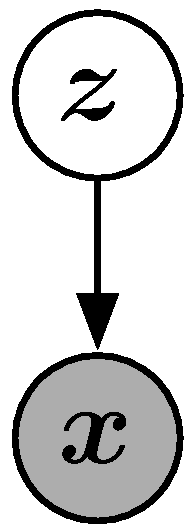
\includegraphics{graph}
  \caption{The graphical model structure of GANs, which is also shared with
    VAEs, sparse coding, etc.
    It is directed graphical model where every latent variable influences
    every observed variable.
    Some GAN variants remove some of these connections.
  }
  \label{fig:graph}
\end{figure}

\subsection{Cost functions}

Several different cost functions may be used within the GANs framework.

\subsubsection{The discriminator's cost, $J^{(D)}$}

All of the different games designed for GANs so far use the same cost for the
discriminator, $J^{(D)}$. They differ only in terms of the cost used for the
generator, $J^{(G)}$.

The cost used for the discriminator is:
\begin{equation}
  J^{(D)}(\vtheta^{(D)}, \vtheta^{(G)}) = -\frac{1}{2} \E_{\vx \sim \pdata} \log D(\vx; \vtheta^{(D)}) - \frac{1}{2} \E_{\vz} \log \left(1 - D\left( G(z); \vtheta^{(G)} \right) \right).
  \label{eq:discriminator_cost}
\end{equation}

This is just the standard cross-entropy cost that is minimized when training a standard binary classifier
with a sigmoid output.
The only difference is that the classifier is trained on two minibatches of data; one coming from the
dataset, where the label is $1$ for all examples, and one coming from the generator, where the label
is $0$ for all examples.


\subsubsection{Minimax}

TODO

